

%% AP Physics MC Questions Archive
%%----------------------------------------


%% Gravitational Potential Energy
%%----------------------------------------
\element{ap}{
\begin{question}{gravitational-potential-energy-q01}
    A block of mass \SI{1}{\kilo\gram} at rest slides down a frictionless inclined plane as shown in the picture.
    \begin{center}
    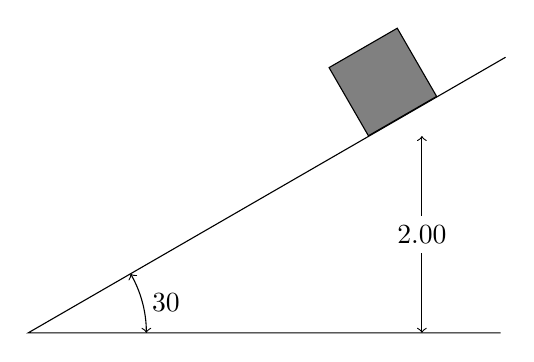
\begin{tikzpicture}
        %% Floor and plane
        \draw (6,0) -- (0,0) -- (30:7);
        %% angle
        \draw[<->] (1.5,0) arc(0:30:1.5) node[pos=0.5,anchor=west] {\ang{30}};
        %% block
        \node[draw,minimum size=1cm,anchor=south east,rotate=30,fill=white!50!black] at (30:6) {};
        %% distance
        %% NOTE: position length label
        \draw[<->] (5,0) -- (5,2.5) node[pos=0.5,anchor=center,fill=white] {\SI{2.00}{\meter}};
    \end{tikzpicture}
    \end{center}
    The plane is sloped at an angle of \ang{30} relative to the ground.
    When the block slides to the ground,
        its change in kinetic energy is most nearly:
    \begin{multicols}{3}
    \begin{choices}
        \wrongchoice{\SI{+10}{\joule}}
        \wrongchoice{\SI{-10}{\joule}}
        \wrongchoice{\SI{+15}{\joule}}
        \wrongchoice{\SI{-15}{\joule}}
      \correctchoice{\SI{+20}{\joule}}
    \end{choices}
    \end{multicols}
\end{question}
}

\element{ap}{
\begin{question}{gravitational-potential-energy-q02}
    %%Base your answer to the following question on the following information.
    A roller coaster car starts at Point $A$ and travels along a frictionless slope traveling to Point $E$ which is at a slightly lower height.
    \begin{center}
    \begin{tikzpicture}
        %% NOTE: TODO: draw tikz
    \end{tikzpicture}
    \end{center}
    The car's speed is the fastest at which point?
    \begin{multicols}{3}
    \begin{choices}[o]
        \wrongchoice{$A$}
        \wrongchoice{$B$}
      \correctchoice{$C$}
        \wrongchoice{$D$}
        \wrongchoice{$E$}
    \end{choices}
    \end{multicols}
\end{question}
}

\element{ap}{
\begin{question}{gravitational-potential-energy-q03}
    %Base your answer to the following question on the diagram below.
    In the diagram, a box of mass $m$ is sliding down a frictionless ramp of length $L$ with an incline of $\theta$ to the horizontal.
    \begin{center}
    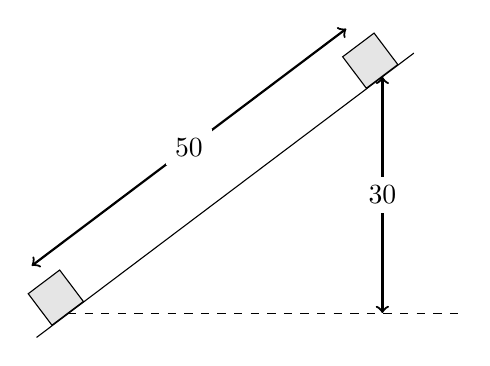
\begin{tikzpicture}
        %% Plane
        \draw (0,0) -- (37:6);
        %% Blocks
        \node[draw,rotate=37,anchor=south,minimum size=0.5cm,fill=white!90!black] (A) at (37:0.5) {};
        \node[draw,rotate=37,anchor=south,minimum size=0.5cm,fill=white!90!black] (B) at (37:5.5) {};
        %% Lables
        \draw[<->,thick] (A.north) ++(127:0.25) -- ++(37:5) node[pos=0.5,anchor=center,fill=white] {\SI{50}{\meter}};
        \draw[<->,thick] (37:5.5) --++(270:3) node[fill=white,pos=0.5,anchor=center] {\SI{30}{\meter}};
        \draw[dashed] (37:0.5) -- ++(0:5);
    \end{tikzpicture}
    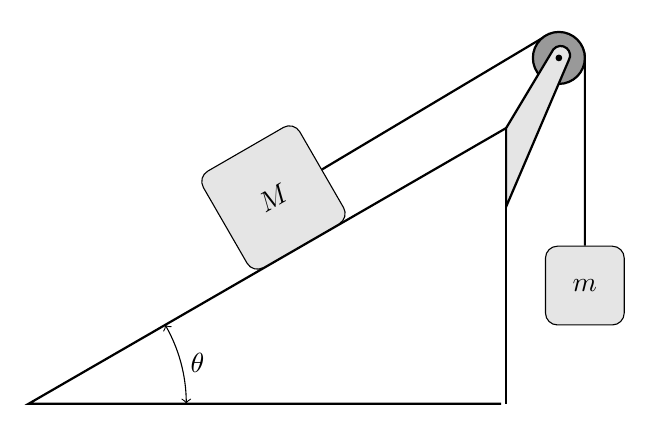
\begin{tikzpicture}
        %% Plane Floor
        \draw[thick] (0,0) -- ++(210:7) -- ++(0:6);
        \draw[<->] (210:7) ++(0:2) arc (0:30:2) node[pos=0.5,anchor=west] {$\theta$};
        \draw[thick] (0,0) -- (270:3.5);
        %% Mass
        \node[draw,fill=white!90!black,rectangle,rounded corners=1ex,minimum size=1.414cm,rotate=30,anchor=south] (A) at (210:3) {$M$};
        \node[draw,fill=white!90!black,rectangle,rounded corners=1ex,minimum size=1cm,anchor=center] (B) at (1,-2) {$m$};
        %% Rope and Pully
        \draw[thick] (A.east) -- (0.505,1.17) arc(120:0:0.33) -- (B.north);
        \draw[thick,fill=white!60!black] (0.67,0.891) circle (0.33);
        \draw[thick,fill=white!90!black] (0,0) -- (0.60,1.0) arc (140:-30:0.12) -- (0,-1) -- cycle;
        \draw[fill] (0.67,0.891) circle (1pt);
    \end{tikzpicture}
    \end{center}
    The mass takes $t$ seconds to slide down the ramp.
    The work done by gravity on the object is equal to:
    \begin{multicols}{2}
    \begin{choices}
        \wrongchoice{$\dfrac{mgL}{t}$}
        \wrongchoice{$\dfrac{mgL\cos\theta}{t}$}
        \wrongchoice{$mgL\cos\theta$}
      \correctchoice{$mgL\sin\theta$}
        \wrongchoice{Cannot be determined from the information given.}
    \end{choices}
    \end{multicols}
\end{question}
}

\element{ap}{
\begin{question}{gravitational-potential-energy-q04}
    In general, if the center of mass of a system is raised to a higher gravitational potential and the system is otherwise unchanged,
    \begin{choices}
        \wrongchoice{the system becomes more stable}
      \correctchoice{the system becomes less stable}
        \wrongchoice{the total energy of the system decreases}
        \wrongchoice{the kinetic energy in the system decreases}
        \wrongchoice{the system does work on its environment}
    \end{choices}
\end{question}
}


\endinput


